\documentclass[fleqn,11pt]{article}

\usepackage[letterpaper,margin=0.75in]{geometry}

\usepackage{amsmath}
\usepackage{booktabs}
\usepackage{graphicx}
\usepackage{listings}

\setlength{\parindent}{1.4em}

\begin{document}

\lstset{
  basicstyle=\small,          % print whole listing small
  keywordstyle=\bfseries,
  identifierstyle=,           % nothing happens
  commentstyle=,              % white comments
  stringstyle=\ttfamily,      % typewriter type for strings
  showstringspaces=false,     % no special string spaces
  numbers=left,
  numberstyle=\tiny,
  numbersep=5pt,
  frame=tb,
}

\title{Network Simulation}

\author{Spencer Wood}

\date{3 Feburary 2016}

\maketitle

\section{Two Nodes}

Three experiments were performed on a two node network using the simulator.
Each experiment measured the delay of a single packet being sent from the
first node $n1$ to the second node $n2$. In each case the packet had a size of
1,000 bytes.

\subsection{Experiment 1}
\vspace{0.5cm}

Listing \ref{lst:two_node_1} shows the network configuration for this experiment.

\vspace{0.5cm}
\begin{lstlisting}[caption={Network configuration},label={lst:two_node_1}]
n1 n2
n2 n1

n1 n2 1Mbps 1seconds
n2 n1 1Mbps 1seconds
\end{lstlisting}
\vspace{0.5cm}

\noindent
Table \ref{tab:two_node_1} shows the simulator output.

\begin{table}[h]
  \caption{Simulator output}
  \label{tab:two_node_1}
  \begin{center}
    \begin{tabular}{cccc}
      \toprule
      Packet ID & Packet Created Time & Packet Received Time & \\
      \midrule
      1 & 0s & 1.008s\\
      \bottomrule
    \end{tabular}
  \end{center}
\end{table}
\vspace{0.5cm}

\noindent
The following calculations were used to verify the accuracy of the simulator:

\begin{align*}
  delay_{total} &= delay_{transmission} + delay_{propagation}\\
  &= \frac{8000bits}{10^6bps} + 1s\\
  &= 0.008s + 1s\\
  &= 1.008s
\end{align*}

\subsection{Experiment 2}
\vspace{0.5cm}

Listing \ref{lst:two_node_2} shows the network configuration for this experiment.

\vspace{0.5cm}
\begin{lstlisting}[caption={Network configuration},label={lst:two_node_2}]
n1 n2
n2 n1

n1 n2 100bps 10ms
n2 n1 100bps 10ms
\end{lstlisting}
\vspace{0.5cm}

\noindent
Table \ref{tab:two_node_2} shows the simulator output.

\begin{table}[h]
  \caption{Simulator output}
  \label{tab:two_node_2}
  \begin{center}
    \begin{tabular}{cccc}
      \toprule
      Packet ID & Packet Created Time & Packet Received Time & \\
      \midrule
      1 & 0s & 80.01s\\
      \bottomrule
    \end{tabular}
  \end{center}
\end{table}
\vspace{0.5cm}

\noindent
The following calculations were used to verify the accuracy of the simulator:

\begin{align*}
  delay_{total} &= delay_{transmission} + delay_{propagation}\\
  &= \frac{8000bits}{100bps} + 0.01s\\
  &= 80s + 0.01s\\
  &= 80.01s
\end{align*}

\subsection{Experiment 3}
\vspace{0.5cm}

In this experiment, four packets were sent from $n1$ to $n2$ at various intervals.\\\\
Listing \ref{lst:two_node_3} shows the network configuration for this experiment.

\vspace{0.5cm}
\begin{lstlisting}[caption={Network configuration},label={lst:two_node_3}]
n1 n2
n2 n1

n1 n2 1Mbps 10ms
n2 n1 1Mbps 10ms
\end{lstlisting}
\vspace{0.5cm}

\vspace{2.5cm}
\noindent
Table \ref{tab:two_node_3} shows the simulator output.

\begin{table}[h]
  \caption{Simulator output}
  \label{tab:two_node_3}
  \begin{center}
    \begin{tabular}{cccc}
      \toprule
      Packet ID & Packet Created Time & Packet Received Time & \\
      \midrule
      1 & 0s & 0.018s\\
      2 & 0s & 0.026s\\
      3 & 0s & 0.034s\\
      4 & 2s & 2.018s\\
      \bottomrule
    \end{tabular}
  \end{center}
\end{table}
\vspace{0.5cm}

\noindent
The following calculations were used to verify the accuracy of the simulator:

\begin{align*}
  delay_{total} &= delay_{transmission} + delay_{propagation}\\
  &= \frac{8000bits}{10^6bps} + 0.01s\\
  &= 0.008s + 0.01s\\
  &= 0.018s
\end{align*}

\noindent
Packets 1, 2, and 3 were all scheduled for $t=0$. Packet 2 must wait for
packet 1 to arrive, and likewise packet 3 must wait for packet 2 to arrive. If
it takes the first packet $0.018s$ to arrive, the next packet will arrive in $2
* 0.018s$ and the next in $3 * 0.018s$.\\

\noindent
Packet 4 was scheduled for $t=2s$ therefore it makes sense that this packet
arrived at $t=2.018s$

\section{Three Nodes}

Two experiments were performed on a three node network using the simulator.
Each experiment measured the delay in sending 1000 packets each of size 1kb
from $n1$ to $n3$.

\subsection{Experiment 1: Two fast links}
\vspace{0.5cm}

Listing \ref{lst:three_node_1_a} shows the network configuration for this experiment.

\vspace{0.5cm}
\begin{lstlisting}[caption={Network configuration},label={lst:three_node_1_a}]
n1 n2
n2 n1 n3
n3 n2

n1 n2 1Mbps 100ms
n2 n1 1Mbps 100ms
n2 n3 1Mbps 100ms
n3 n2 1Mbps 100ms
\end{lstlisting}

\pagebreak

\noindent
Table \ref{tab:three_node_1_a} shows the simulator output.

\begin{table}[h]
  \caption{Simulator output}
  \label{tab:three_node_1_a}
  \begin{center}
    \begin{tabular}{cccc}
      \toprule
      Packet ID & Packet Created Time & Packet Received Time & \\
      \midrule
      1 & 0 & 0.216\\
      ... & ... & ...\\
      996 & 7.96 & 8.176\\
      997 & 7.968 & 8.184\\
      998 & 7.976 & 8.192\\
      999 & 7.984 & 8.200\\
      1000 & 7.992 & 8.208\\
      \bottomrule
    \end{tabular}
  \end{center}
\end{table}
\vspace{0.5cm}

\noindent
The following calculations were used to verify the accuracy of the simulator:\\

Packets were queued as soon as the previous packet's transmission delay was up.

\begin{align*}
  delay_{total} &= 2 * (delay_{transmission} + delay_{propagation})\\
  &= \frac{8000bits}{10^6mbps} + 0.1s\\
  &= 0.008s + 0.1s\\
  &= 0.108s
\end{align*}

\noindent
The above calculation is for the first packet. For any other packet it is
necessary to add \\ $(i - 1) * transmission_{delay}$ where $i$ is the packet
number. For example packet 999 the calculation would be $998 * 0.008s +
2(0.108s) = 8.2s$ \\

If we increase the bandwidth to 1Gbps on each link we get the following results
shown in Table \ref{tab:three_node_1_b}

\begin{table}[h]
  \caption{Simulator output}
  \label{tab:three_node_1_b}
  \begin{center}
    \begin{tabular}{cccc}
      \toprule
      Packet ID & Packet Created Time & Packet Received Time & \\
      \midrule
      1 & 0 & 0.200016\\
      ... & ... & ...\\
      996 & 0.00796 & 0.207976\\
      997 & 0.007968 & 0.207984\\
      998 & 0.007976 & 0.207992\\
      999 & 0.007984 & 0.208000\\
      1000 & 0.007992 & 0.208008\\
      \bottomrule
    \end{tabular}
  \end{center}
\end{table}
\vspace{0.5cm}

\pagebreak


\subsection{Experiment 2: One Fast One Slow}
\vspace{0.5cm}

Listing \ref{lst:three_node_2} shows the network configuration for this experiment.

\vspace{0.5cm}
\begin{lstlisting}[caption={Network configuration},label={lst:three_node_2}]
n1 n2
n2 n1 n3
n3 n2

n1 n2 1Mbps 100ms
n2 n1 1Mbps 100ms
n2 n3 256Kbps 100ms
n3 n2 256Kbps 100ms
\end{lstlisting}

\noindent
Table \ref{tab:three_node_2} shows the simulator output.

\begin{table}[h]
  \caption{Simulator output}
  \label{tab:three_node_2}
  \begin{center}
    \begin{tabular}{cccc}
      \toprule
      Packet ID & Packet Created Time & Packet Received Time & \\
      \midrule
      1 & 0 & 0.23925\\
      ... & ... & ...\\
      996 & 7.96 & 31.333\\
      997 & 7.968 & 31.36425\\
      998 & 7.976 & 31.3955\\
      999 & 7.984 & 31.42675\\
      1000 & 7.992 & 31.458\\
      \bottomrule
    \end{tabular}
  \end{center}
\end{table}
\vspace{0.5cm}

\noindent
The calculations for this part are similar to those in part 1 however instead
of multiplying the transmission delay and propagation delay by two, it is
necessary to calculate the propagation and transmission delay of each link and
apply it to each packet being sent.

\begin{align*}
  delay_{link1} &= 0.008s + 0.1s\\
  delay_{link2} &= 0.03125s + 0.1s\\
  delay_{total} &= 0.23925s\\
\end{align*}

\noindent
Again, the above calcuation applies to the first packet. To calculate the delay
for an arbitrary packet one must add $((i - 1) * delay_{transmission})$ to $delay_{total}$ where
$i$ is the packet number.

\section{Queueing Theory}
\vspace{0.5cm}

The simulator was used to valid basic query that shows that as utilization goes
up the queueing time approaches infinity.\\

\pagebreak
Listing \ref{lst:queing_theory} shows the network configuration for this experiment.

\vspace{0.5cm}
\begin{lstlisting}[caption={Network configuration},label={lst:queing_theory}]
n1 n2
n2 n1

n1 n2 1Mbps 1ms
n2 n1 1Mbps 1ms
\end{lstlisting}
\vspace{0.5cm}


\noindent
We ran the simulator with the following utilization loads: .1, .2, .3, .4, .5,
.6, .7, .8, .9, .95, .98\\

\noindent
Table \ref{tab:queing_theory} shows the simulator output.

\begin{table}[h]
  \caption{Simulator output}
  \label{tab:queing_theory}
  \begin{center}
    \begin{tabular}{cccc}
      \toprule
      Queueing Delay & Utilization & \\
      \midrule
      0.1 & 0.00039723538144099095\\
      0.2 & 0.0009259551823570379\\
      0.3 & 0.0015353808146987397\\
      0.4 & 0.0022040796728314584\\
      0.5 & 0.0040643837154374285\\
      0.6 & 0.005178718239070869\\
      0.7 & 0.010346967801745273\\
      0.8 & 0.014725987301735601\\
      0.9 & 0.02507878037089064\\
      0.95 & 0.1214653059329094\\
      0.98 & 0.2499052036096885\\
      \bottomrule
    \end{tabular}
  \end{center}
\end{table}

\noindent
The graph below shows the simulator output in relation to the theoretical
equation that shows queueing delay approach infinity. The result is two lines
that match well.

\begin{center}
  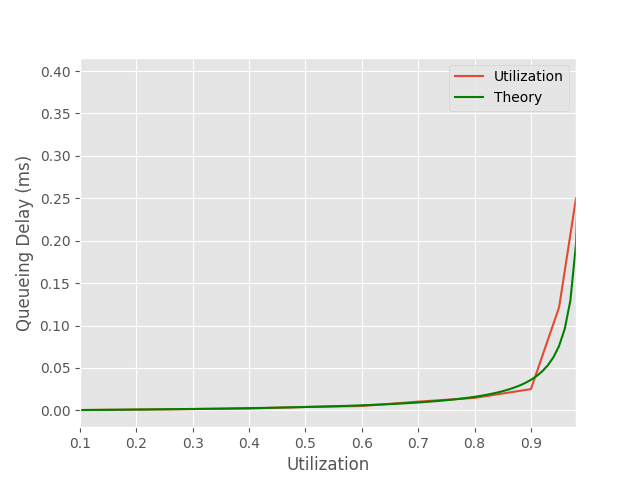
\includegraphics[width=11cm]{queueing_theory}
\end{center}

\end{document}
